%% bare_jrnl_transmag.tex
%% V1.4b
%% 2015/08/26
%% by Michael Shell
%% see http://www.michaelshell.org/
%% for current contact information.
%%
%% This is a skeleton file demonstrating the use of IEEEtran.cls
%% (requires IEEEtran.cls version 1.8b or later) with an IEEE 
%% Transactions on Magnetics journal paper.
%%
%% Support sites:
%% http://www.michaelshell.org/tex/ieeetran/
%% http://www.ctan.org/pkg/ieeetran
%% and
%% http://www.ieee.org/

%%*************************************************************************
%% Legal Notice:
%% This code is offered as-is without any warranty either expressed or
%% implied; without even the implied warranty of MERCHANTABILITY or
%% FITNESS FOR A PARTICULAR PURPOSE! 
%% User assumes all risk.
%% In no event shall the IEEE or any contributor to this code be liable for
%% any damages or losses, including, but not limited to, incidental,
%% consequential, or any other damages, resulting from the use or misuse
%% of any information contained here.
%%
%% All comments are the opinions of their respective authors and are not
%% necessarily endorsed by the IEEE.
%%
%% This work is distributed under the LaTeX Project Public License (LPPL)
%% ( http://www.latex-project.org/ ) version 1.3, and may be freely used,
%% distributed and modified. A copy of the LPPL, version 1.3, is included
%% in the base LaTeX documentation of all distributions of LaTeX released
%% 2003/12/01 or later.
%% Retain all contribution notices and credits.
%% ** Modified files should be clearly indicated as such, including  **
%% ** renaming them and changing author support contact information. **
%%*************************************************************************


% *** Authors should verify (and, if needed, correct) their LaTeX system  ***
% *** with the testflow diagnostic prior to trusting their LaTeX platform ***
% *** with production work. The IEEE's font choices and paper sizes can   ***
% *** trigger bugs that do not appear when using other class files.       ***                          ***
% The testflow support page is at:
% http://www.michaelshell.org/tex/testflow/



\documentclass[journal,transmag]{IEEEtran}
%
% If IEEEtran.cls has not been installed into the LaTeX system files,
% manually specify the path to it like:
% \documentclass[journal]{../sty/IEEEtran}




% Some very useful LaTeX packages include:
% (uncomment the ones you want to load)


% *** MISC UTILITY PACKAGES ***
%
%\usepackage{ifpdf}
% Heiko Oberdiek's ifpdf.sty is very useful if you need conditional
% compilation based on whether the output is pdf or dvi.
% usage:
% \ifpdf
%   % pdf code
% \else
%   % dvi code
% \fi
% The latest version of ifpdf.sty can be obtained from:
% http://www.ctan.org/pkg/ifpdf
% Also, note that IEEEtran.cls V1.7 and later provides a builtin
% \ifCLASSINFOpdf conditional that works the same way.
% When switching from latex to pdflatex and vice-versa, the compiler may
% have to be run twice to clear warning/error messages.






% *** CITATION PACKAGES ***
%
%\usepackage{cite}
% cite.sty was written by Donald Arseneau
% V1.6 and later of IEEEtran pre-defines the format of the cite.sty package
% \cite{} output to follow that of the IEEE. Loading the cite package will
% result in citation numbers being automatically sorted and properly
% "compressed/ranged". e.g., [1], [9], [2], [7], [5], [6] without using
% cite.sty will become [1], [2], [5]--[7], [9] using cite.sty. cite.sty's
% \cite will automatically add leading space, if needed. Use cite.sty's
% noadjust option (cite.sty V3.8 and later) if you want to turn this off
% such as if a citation ever needs to be enclosed in parenthesis.
% cite.sty is already installed on most LaTeX systems. Be sure and use
% version 5.0 (2009-03-20) and later if using hyperref.sty.
% The latest version can be obtained at:
% http://www.ctan.org/pkg/cite
% The documentation is contained in the cite.sty file itself.
\usepackage{cite}
\usepackage[colorlinks=true, allcolors=blue, pagebackref=true]{hyperref}
\usepackage[font=small,labelfont=bf,justification=centering]{caption}




% *** GRAPHICS RELATED PACKAGES ***
%
\ifCLASSINFOpdf
  % \usepackage[pdftex]{graphicx}
  % declare the path(s) where your graphic files are
  % \graphicspath{{../pdf/}{../jpeg/}}
  % and their extensions so you won't have to specify these with
  % every instance of \includegraphics
  % \DeclareGraphicsExtensions{.pdf,.jpeg,.png}
\else
  % or other class option (dvipsone, dvipdf, if not using dvips). graphicx
  % will default to the driver specified in the system graphics.cfg if no
  % driver is specified.
  % \usepackage[dvips]{graphicx}
  % declare the path(s) where your graphic files are
  % \graphicspath{{../eps/}}
  % and their extensions so you won't have to specify these with
  % every instance of \includegraphics
  % \DeclareGraphicsExtensions{.eps}
\fi
% graphicx was written by David Carlisle and Sebastian Rahtz. It is
% required if you want graphics, photos, etc. graphicx.sty is already
% installed on most LaTeX systems. The latest version and documentation
% can be obtained at: 
% http://www.ctan.org/pkg/graphicx
% Another good source of documentation is "Using Imported Graphics in
% LaTeX2e" by Keith Reckdahl which can be found at:
% http://www.ctan.org/pkg/epslatex
%
% latex, and pdflatex in dvi mode, support graphics in encapsulated
% postscript (.eps) format. pdflatex in pdf mode supports graphics
% in .pdf, .jpeg, .png and .mps (metapost) formats. Users should ensure
% that all non-photo figures use a vector format (.eps, .pdf, .mps) and
% not a bitmapped formats (.jpeg, .png). The IEEE frowns on bitmapped formats
% which can result in "jaggedy"/blurry rendering of lines and letters as
% well as large increases in file sizes.
%
% You can find documentation about the pdfTeX application at:
% http://www.tug.org/applications/pdftex

\usepackage{amssymb}   % make sure this is in your preamble
\usepackage{booktabs}  % optional but cleaner rules
\usepackage{graphicx}
\usepackage{tikz}
\usetikzlibrary{shapes.geometric, arrows.meta, positioning}
\usepackage{amsmath}


% *** MATH PACKAGES ***
%
%\usepackage{amsmath}
% A popular package from the American Mathematical Society that provides
% many useful and powerful commands for dealing with mathematics.
%
% Note that the amsmath package sets \interdisplaylinepenalty to 10000
% thus preventing page breaks from occurring within multiline equations. Use:
%\interdisplaylinepenalty=2500
% after loading amsmath to restore such page breaks as IEEEtran.cls normally
% does. amsmath.sty is already installed on most LaTeX systems. The latest
% version and documentation can be obtained at:
% http://www.ctan.org/pkg/amsmath





% *** SPECIALIZED LIST PACKAGES ***
%
%\usepackage{algorithmic}
% algorithmic.sty was written by Peter Williams and Rogerio Brito.
% This package provides an algorithmic environment fo describing algorithms.
% You can use the algorithmic environment in-text or within a figure
% environment to provide for a floating algorithm. Do NOT use the algorithm
% floating environment provided by algorithm.sty (by the same authors) or
% algorithm2e.sty (by Christophe Fiorio) as the IEEE does not use dedicated
% algorithm float types and packages that provide these will not provide
% correct IEEE style captions. The latest version and documentation of
% algorithmic.sty can be obtained at:
% http://www.ctan.org/pkg/algorithms
% Also of interest may be the (relatively newer and more customizable)
% algorithmicx.sty package by Szasz Janos:
% http://www.ctan.org/pkg/algorithmicx




% *** ALIGNMENT PACKAGES ***
%
%\usepackage{array}
% Frank Mittelbach's and David Carlisle's array.sty patches and improves
% the standard LaTeX2e array and tabular environments to provide better
% appearance and additional user controls. As the default LaTeX2e table
% generation code is lacking to the point of almost being broken with
% respect to the quality of the end results, all users are strongly
% advised to use an enhanced (at the very least that provided by array.sty)
% set of table tools. array.sty is already installed on most systems. The
% latest version and documentation can be obtained at:
% http://www.ctan.org/pkg/array


% IEEEtran contains the IEEEeqnarray family of commands that can be used to
% generate multiline equations as well as matrices, tables, etc., of high
% quality.




% *** SUBFIGURE PACKAGES ***
%\ifCLASSOPTIONcompsoc
%  \usepackage[caption=false,font=normalsize,labelfont=sf,textfont=sf]{subfig}
%\else
%  \usepackage[caption=false,font=footnotesize]{subfig}
%\fi
% subfig.sty, written by Steven Douglas Cochran, is the modern replacement
% for subfigure.sty, the latter of which is no longer maintained and is
% incompatible with some LaTeX packages including fixltx2e. However,
% subfig.sty requires and automatically loads Axel Sommerfeldt's caption.sty
% which will override IEEEtran.cls' handling of captions and this will result
% in non-IEEE style figure/table captions. To prevent this problem, be sure
% and invoke subfig.sty's "caption=false" package option (available since
% subfig.sty version 1.3, 2005/06/28) as this is will preserve IEEEtran.cls
% handling of captions.
% Note that the Computer Society format requires a larger sans serif font
% than the serif footnote size font used in traditional IEEE formatting
% and thus the need to invoke different subfig.sty package options depending
% on whether compsoc mode has been enabled.
%
% The latest version and documentation of subfig.sty can be obtained at:
% http://www.ctan.org/pkg/subfig



% *** FLOAT PACKAGES ***
%
%\usepackage{fixltx2e}
% fixltx2e, the successor to the earlier fix2col.sty, was written by
% Frank Mittelbach and David Carlisle. This package corrects a few problems
% in the LaTeX2e kernel, the most notable of which is that in current
% LaTeX2e releases, the ordering of single and double column floats is not
% guaranteed to be preserved. Thus, an unpatched LaTeX2e can allow a
% single column figure to be placed prior to an earlier double column
% figure.
% Be aware that LaTeX2e kernels dated 2015 and later have fixltx2e.sty's
% corrections already built into the system in which case a warning will
% be issued if an attempt is made to load fixltx2e.sty as it is no longer
% needed.
% The latest version and documentation can be found at:
% http://www.ctan.org/pkg/fixltx2e


%\usepackage{stfloats}
% stfloats.sty was written by Sigitas Tolusis. This package gives LaTeX2e
% the ability to do double column floats at the bottom of the page as well
% as the top. (e.g., "\begin{figure*}[!b]" is not normally possible in
% LaTeX2e). It also provides a command:
%\fnbelowfloat
% to enable the placement of footnotes below bottom floats (the standard
% LaTeX2e kernel puts them above bottom floats). This is an invasive package
% which rewrites many portions of the LaTeX2e float routines. It may not work
% with other packages that modify the LaTeX2e float routines. The latest
% version and documentation can be obtained at:
% http://www.ctan.org/pkg/stfloats
% Do not use the stfloats baselinefloat ability as the IEEE does not allow
% \baselineskip to stretch. Authors submitting work to the IEEE should note
% that the IEEE rarely uses double column equations and that authors should try
% to avoid such use. Do not be tempted to use the cuted.sty or midfloat.sty
% packages (also by Sigitas Tolusis) as the IEEE does not format its papers in
% such ways.
% Do not attempt to use stfloats with fixltx2e as they are incompatible.
% Instead, use Morten Hogholm'a dblfloatfix which combines the features
% of both fixltx2e and stfloats:
%
% \usepackage{dblfloatfix}
% The latest version can be found at:
% http://www.ctan.org/pkg/dblfloatfix




%\ifCLASSOPTIONcaptionsoff
%  \usepackage[nomarkers]{endfloat}
% \let\MYoriglatexcaption\caption
% \renewcommand{\caption}[2][\relax]{\MYoriglatexcaption[#2]{#2}}
%\fi
% endfloat.sty was written by James Darrell McCauley, Jeff Goldberg and 
% Axel Sommerfeldt. This package may be useful when used in conjunction with 
% IEEEtran.cls'  captionsoff option. Some IEEE journals/societies require that
% submissions have lists of figures/tables at the end of the paper and that
% figures/tables without any captions are placed on a page by themselves at
% the end of the document. If needed, the draftcls IEEEtran class option or
% \CLASSINPUTbaselinestretch interface can be used to increase the line
% spacing as well. Be sure and use the nomarkers option of endfloat to
% prevent endfloat from "marking" where the figures would have been placed
% in the text. The two hack lines of code above are a slight modification of
% that suggested by in the endfloat docs (section 8.4.1) to ensure that
% the full captions always appear in the list of figures/tables - even if
% the user used the short optional argument of \caption[]{}.
% IEEE papers do not typically make use of \caption[]'s optional argument,
% so this should not be an issue. A similar trick can be used to disable
% captions of packages such as subfig.sty that lack options to turn off
% the subcaptions:
% For subfig.sty:
% \let\MYorigsubfloat\subfloat
% \renewcommand{\subfloat}[2][\relax]{\MYorigsubfloat[]{#2}}
% However, the above trick will not work if both optional arguments of
% the \subfloat command are used. Furthermore, there needs to be a
% description of each subfigure *somewhere* and endfloat does not add
% subfigure captions to its list of figures. Thus, the best approach is to
% avoid the use of subfigure captions (many IEEE journals avoid them anyway)
% and instead reference/explain all the subfigures within the main caption.
% The latest version of endfloat.sty and its documentation can obtained at:
% http://www.ctan.org/pkg/endfloat
%
% The IEEEtran \ifCLASSOPTIONcaptionsoff conditional can also be used
% later in the document, say, to conditionally put the References on a 
% page by themselves.




% *** PDF, URL AND HYPERLINK PACKAGES ***
%
%\usepackage{url}
% url.sty was written by Donald Arseneau. It provides better support for
% handling and breaking URLs. url.sty is already installed on most LaTeX
% systems. The latest version and documentation can be obtained at:
% http://www.ctan.org/pkg/url
% Basically, \url{my_url_here}.




% *** Do not adjust lengths that control margins, column widths, etc. ***
% *** Do not use packages that alter fonts (such as pslatex).         ***
% There should be no need to do such things with IEEEtran.cls V1.6 and later.
% (Unless specifically asked to do so by the journal or conference you plan
% to submit to, of course. )


% correct bad hyphenation here
\hyphenation{op-tical net-works semi-conduc-tor}


\begin{document}
%
% paper title
% Titles are generally capitalized except for words such as a, an, and, as,
% at, but, by, for, in, nor, of, on, or, the, to and up, which are usually
% not capitalized unless they are the first or last word of the title.
% Linebreaks \\ can be used within to get better formatting as desired.
% Do not put math or special symbols in the title.
\title{A Unified Multimodal Framework for Mushroom Identification}

% author names and affiliations
% transmag papers use the long conference author name format.

\author{\IEEEauthorblockN{Victor Hugo Figueroa\IEEEauthorrefmark{1},
Herman Klausen Skoglund\IEEEauthorrefmark{2},and 
Chonthichar Soythong\IEEEauthorrefmark{3}~\IEEEmembership{}}
\IEEEauthorblockA{\IEEEauthorrefmark{1}Oslo Metropolitan University}

\thanks{}}



% The paper headers
% \markboth{Journal of \LaTeX\ Class Files,~Vol.~14, No.~8, August~2015}%
% {Shell \MakeLowercase{\textit{et al.}}: Multimodal Mushroom Classification}
% The only time the second header will appear is for the odd numbered pages
% after the title page when using the twoside option.
% 
% *** Note that you probably will NOT want to include the author's ***
% *** name in the headers of peer review papers.                   ***
% You can use \ifCLASSOPTIONpeerreview for conditional compilation here if
% you desire.




% If you want to put a publisher's ID mark on the page you can do it like
% this:
%\IEEEpubid{0000--0000/00\$00.00~\copyright~2015 IEEE}
% Remember, if you use this you must call \IEEEpubidadjcol in the second
% column for its text to clear the IEEEpubid mark.

\renewenvironment{IEEEkeywords}{}{}

% use for special paper notices
%\IEEEspecialpapernotice{(Invited Paper)}


% for Transactions on Magnetics papers, we must declare the abstract and
% index terms PRIOR to the title within the \IEEEtitleabstractindextext
% IEEEtran command as these need to go into the title area created by
% \maketitle.
% As a general rule, do not put math, special symbols or citations
% in the abstract or keywords.
\IEEEtitleabstractindextext{%
\begin{abstract}
Traditionaly, automated mushroom identification has been a unimodal classification task, where most systems predict only species labels
and confidence scores from a single image. This single-modality
approaches lacks ecological grounding, language-based reasoning, and interpretable outputs, limiting their usefullness in real-world context, where
misidentification can result in severe health consequences. In this
study, we propose a unified multimodal mushroom identification
framework based on a four-stage pipeline: (1) computer vision
classification, (2) ecological context retrieval, (3) Large Language
Model (LLM) audit reasoning, and (4) interpretable output generation, implemented as a complete end-to-end deployable system.
six model architectures were evaluated int this study across 169 species and approximately
689,000 images. YOLOv26n-cls was selected as the deployment model,
achieving 88.1\% Top-1 and 98.4\% Top-5 accuracy with 4.8\,ms CPU
inference via TFLite export. An ablation study showed that standalone vision models missed between 70.0\% and 85.7\% of dangerous cases, however adding the Gemini LLM assessment layer improved recall for detecting toxic and dangerous species from
30.0\% to 75.9\%, with a false positive rate of 18.6\% and an F1
score of 80.0\%. The structured multimodal output additionally expands the identification report from 2 fields in a standard classifier to 13 fields, including toxicity class, ecological database, risk level of the mushrooms,  and plain-language recommendations. These results indicate that the proposed  four-stages pipeline produces more informative and interpretable outputs than using only vision modals. The system is deployed as a web application via \href{https://brain-ui-849718487429.us-central1.run.app}{Google Cloud Run} 
and code is available on \href{https://github.com/QuasimodoCodes/Mushrooms/tree/master}{GitHub}.
\end{abstract}

% Note that keywords are not normally used for peerreview papers.
\begin{IEEEkeywords}
\end{IEEEkeywords}}



% make the title area
\maketitle


% To allow for easy dual compilation without having to reenter the
% abstract/keywords data, the \IEEEtitleabstractindextext text will
% not be used in maketitle, but will appear (i.e., to be "transported")
% here as \IEEEdisplaynontitleabstractindextext when the compsoc 
% or transmag modes are not selected <OR> if conference mode is selected 
% - because all conference papers position the abstract like regular
% papers do.
\IEEEdisplaynontitleabstractindextext
% \IEEEdisplaynontitleabstractindextext has no effect when using
% compsoc or transmag under a non-conference mode.







% For peer review papers, you can put extra information on the cover
% page as needed:
% \ifCLASSOPTIONpeerreview
% \begin{center} \bfseries EDICS Category: 3-BBND \end{center}
% \fi
%
% For peerreview papers, this IEEEtran command inserts a page break and
% creates the second title. It will be ignored for other modes.
\IEEEpeerreviewmaketitle



\section{\textbf{Introduction}}
% The very first letter is a 2 line initial drop letter followed
% by the rest of the first word in caps.
% 
% form to use if the first word consists of a single letter:
% \IEEEPARstart{A}{demo} file is ....
% 
% form to use if you need the single drop letter followed by
% normal text (unknown if ever used by the IEEE):
% \IEEEPARstart{A}{}demo file is ....
% 
% Some journals put the first two words in caps:
% \IEEEPARstart{T}{his demo} file is ....
% 
% Here we have the typical use of a "T" for an initial drop letter
% and "HIS" in caps to complete the first word.
\subsection{Background and Problem Statement}

\IEEEPARstart{M}{ushrooms} represent a growing area of scientific and commercial interest, with applications ranging from the food industry to biopharmaceutical development\cite{mayirnao2025}. However, distinguishing between mushroom species remains difficult due to the fine-grained nature of their physical features between certain species\cite{sevindik2025}. 

In the real-world, certain poisonous or edible mushroom species can appear nearly identical to the untrained eye, so that misidentifying them can therefore lead to fatal consequences. The challenge is further compounded by the fact that mushroom appearance changes with age, weather exposure, and geographic conditions, which is reducing the reliability of identification based solely on visual inspection\cite{picek2025fungitastic}.

Existing research has explored a range of architectures, including convolutional neural networks, residual networks, transformers and object detection models, demonstrating promising prediction under controlled experimental settings\cite{kuznetsov2026}. Despite the growing availability of deep leaning mushroom identification tools, most existing research papers recognized mushrooms as a standard image classification task, predicting only species labels and a numerical confidence score from a single photograph.
 
 These outputs are generated without consideration of ecological factors such as habitat, season, or geographic location, even though such factors may be relevant when distinguishing between visually similar species and assessing the risk \cite{picek2025fungitastic}. 
 
 Furthermore, current systems rarely provide reasoning behind the prediction to support user understanding. As a 
 result, they remain limited in practical transparency and decision support capability, particularly when the identification involves edible and toxic mushroom species\cite{kuznetsov2026}.

To address these limitations, we propose a unified multimodal mushroom identification framework that integrates computer vision, structured ecological knowledge, and large language model reasoning as a complete end-to-end system, with the primary aim of providing more interpretable identification support than purely visual classification.
% You must have at least 2 lines in the paragraph with the drop letter
% (should never be an issue)


% needed in second column of first page if using \IEEEpubid
%\IEEEpubidadjcol

\subsection{\textbf{Research Questions}}
This study addresses the following research questions, which correspond directly to the identified research gaps: 

\textbf{{RQ1:}} Which computer vision architecture provides the best trade-off between classification accuracy and deployment efficiently across 169 species?

\textbf{{RQ2:}} Does the selected deployment model generalise competitively on an external mushroom classification benchmark beyond the primary dataset?

\textbf{{RQ3:}} Does adding ecological context and LLM audit layer improve the detection of potentially dangerous mushroom cases compared with unimodal visual classification?

\textbf{{RQ4:}} Does a structured multimodal output schema provide more  interpretable and useful identification support than a standard classifier output containing only a species label and confidence score?

\subsection{\textbf{Contributions}}
\textbf{This study makes the following contributions: }


\subsubsection{A deployable multimodal identification pipeline.} We propose and implement a four-stage pipeline integrating computer vision classification, ecological context retrieval, LLM audit reasoning, and deterministic risk assessment into a single end-to-end deployable system.  

\subsubsection{A systematic evaluation.} We evaluate the pipeline through internal benchmarking of three architectures across 169 species, external validation on the DF24-Mini benchmark, and an ablation study comparing image-only classification, standalone Gemini, and multimodal configurations.



% ------ Related Work ------
\section{\textbf{Related Work}}
\subsection{Traditional Mushroom Identification}

Mushroom identification has traditionally relied on visual observation and expert mycological assessment. More recently, research has shifted toward rule-based systems, machine learning, and deep learning classifiers to identify mushrooms directly from images. However, systems based only on visual input remain limited in real-world  contexts because they do not fully account for ecological conditions or provide sufficient explanation for the prediction~\cite{kuznetsov2026}.


\subsection{Mushroom Species Classification Using Computer Vision}
Computer vision has become a common approach for mushroom species classification, particularity as deep learning models can learn visual features such as color, shape, texture and structural patterns. Previous studies have evaluated CNN-based architectures such as  DenseNet121,  EfficientNet-B0, MobileNetV3, and Shuffle-net for fungi classification\cite{korkmaz2025}\cite{ozsari2024}. This development has moved beyond static classification toward real time detection including edge deployment and toxic species, \cite{duman2025}\cite{wei2025pmyolo}.
 Among transfer and hybrid approaches Swin Transformer and a multimodal MDF-DETR architecture have been explored, though transformer found underperformed CNN baseline on small fungi dataset\cite{ozsari2024}\cite{wang2025mdfdetr}. 
 

\subsection{\textbf{Ecological and Contextual Factors}}
A significant challenge in mushroom classification is that many systems relies mainly on visual images, while ecological information such as habitat, season, geographic region, and toxicity is rarely used as part of the identification process\cite{picek2025fungitastic}. This is important because visually similar mushroom species may differ in where and when they grow, as well as in their toxicological risk \cite{kuznetsov2026}. 

Picek et al.\cite{picek2022danishfungi} introduced the Danish Fungi 2020 dataset (DF24-Mini split), an expert-verified dataset with temporal metadata across a wide range of species which is use in this study for external validation. Recently, Picek et al. \cite{picek2025fungitastic} furthers published baseline metrics for state-of-the-art architectures on this exact dataset. Their FungiTastic benchmark further shows that visual classification alone achieves only 40\% F1 and remains unrealistic at taxonomic scale, providing strong motivation for integrating ecological context into the pipeline \cite{picek2025fungitastic}. 

\subsection{\textbf{Explainability and Decision Support}}

The black-box nature of deep learning remains a challenge in mushroom identification.

 Within the mushroom literature, previous studies have applied visual explanation methods such as Grad-CAM, Score-CAM, and Integrated Gradients to show which image regions influenced the prediction \cite{sevindik2025}\cite{korkmaz2025}\cite{ozsari2024}. These technique can improve transparency by highlighting the important visual areas, but a heatmap alone cannot explains ecological plausibility, possible lookalikes species, toxicity and why a prediction should be trusted.

Studies on toxic mushroom detection still only predict toxic species with class labels and bounding boxes but provides limited information for interpreting the result \cite{wei2025pmyolo}.


\subsection{Summary of Gaps}
Despite recent advances in deep learning for automated mushroom species classification, several challenges remain unsolved.

First, prior systems rely solely on single images, which are insufficient to distinguish visually similar toxic and edible species, and therefore remain limited in practical capability\cite{picek2025fungitastic}\cite{kuznetsov2026}. 

Second, to our knowledge, no existing system integrates ecological context such as, season, habitat, geographic range and mycological habitat constraints into the model’s identification pipeline for edible and toxic mushroom assessment. While, Picek 
et al.~\cite{picek2025fungitastic} integrated introduce an image dataset that includes habitat, substrate, and season metadata, their focus remains on species recognition accuracy rather than toxicity risk assessment, leaving predictions ecologically ungrounded\cite{wei2025pmyolo}. 

Third, most systems operate as black-box classifiers that provide only prediction scores without reasoning behind that prediction, leaving users unable to assess why a prediction was made\cite{sevindik2025}\cite{korkmaz2025}\cite{ozsari2024}. 

Table~\ref{tab:related-comparison} summaries these gaps across the six most relevant prior systems and shows that no prior works integrates all five systems addressed in this study.

\begin{table}[h]
\centering
\small
\caption{Comparison of prior mushroom classification systems 
across key capabilities.}
\label{tab:related-comparison}
\setlength{\tabcolsep}{4pt}
\begin{tabular}{lccccc}
\hline
\textbf{System} & \textbf{Vision} & \textbf{Ecological} & 
\textbf{LLM} & \textbf{Safety} & \textbf{Explainable} \\
 & & \textbf{Context} & 
\textbf{Audit} & \textbf{Output} & \textbf{AI} \\
\hline
Sevindik et al.~\cite{sevindik2025}  
& \checkmark & x & x & x & \checkmark \\
Korkmaz et al.~\cite{korkmaz2025}   
& \checkmark & x & x & x & \checkmark \\
Ozsari et al.~\cite{ozsari2024}     
& \checkmark & x & x & x & x \\
Wei et al.~\cite{wei2025pmyolo}           
& \checkmark & x & x & x & x \\
Picek et al.~\cite{picek2025fungitastic}       
& \checkmark & \checkmark & x & x & x \\
\textbf{Ours}                       
& \checkmark & \checkmark & \checkmark & \checkmark & \checkmark \\
\hline
\end{tabular}
\end{table}

% ------ METHODOLOGY ------
\section{\textbf{Methodology}}
\subsection{\textbf{Overview}}
The methodology is structured around the four research questions and consists of three main experimental components.

First, a systematic vision model benchmark was conducted to address RQ1. Three architecturally 
distinct models were trained and evaluated on the same 169-species dataset. YOLOv26n-cls was additionally evaluated on the external DF24-Mini benchmark to address RQ2.

Second, an ablation study was conducted to address RQ3, investigating whether adding ecological context and an LLM audit layer improves the detection of potentially dangerous mushroom cases compared with unimodal visual classification. 

Third, a structured output comparison was conducted to address RQ4, evaluating the interpretable of the proposed multimodal pipeline compared to a standard vision classification models.

In the production pipeline, YOLOv26n-cls generates a species prediction from the input image, which is passed through a four-stage pipeline combining ecological context retrieval, LLM audit reasoning, and deterministic risk classification to produce the final structured output.

\subsection{\textbf{Dataset}}

\subsubsection{\textbf{Mushroom Species Recognition Image Dataset}}
All models were trained and evaluated on a dataset of 169 mushroom species comprising approximately 689,000 images sourced from Kaggle \textit{Mushroom species recognition} \cite{kaggle_mushroom1}. Images were partitioned into an 80/10/10 train/validation/ and test split, with all models evaluated on the same held-out test set to ensure a fair comparison. The classification task was formulated as single-label supervised image classification, where each image is mapped to exactly one species label.

\subsubsection{\textbf{Danish Fungi image dataset}}
The Danish Fungi dataset was introduced as a fine-grained fungal image-recognition benchmark with expert-verified labels and rich observation metadata, including geographic, habitat, and substrate information\cite{picek2022danishfungi}\cite{picek2025fungitastic}. In this study, the DF24-Mini benchmark is used for external validation.

\subsubsection{\textbf{Ecological Database}}\label{sec:ecological-db}
To support multimodal pipeline, ecological metadata was compiled into a structured JSON database containing 12 fields per species, including toxicity classification, habitat, season, geographic region, morphological descriptions, known lookalike species, and foraging guidance. The database examples are provided in Appendix ~\ref{app:eco-schema}. These records were compiled primarily from multiple open-source Wikipedia species articles and the iNaturalist open-access taxonomy database, which were used to verify species names and ecological data\cite{wikipedia_mushroom}\cite{inaturalist_taxa}. 

It is acknowledged that these records have not been independently verified against primary mycological sources and should therefore be used as a prototype knowledge base only. 


\subsection{\textbf{Vision Model Benchmarking}}

Eight computer vision architectures were initially explored to identify a suitable model for production deployment. Base on this literature, we select three distinct architecture for systematic benchmarking, YOLOv26n-cls as a lightweight detection-derived  classifier, ConvNeXt-Tiny as a modern CNN baseline, and DINOv2-Small as a self-supervised vision transformer. A full configuration is provided in 
Appendix~\ref{app:full-bench}, 
Table~\ref{tab:full-leaderboard}. 


\textbf{YOLOv26n-cls} is a lightweight YOLO-based image classier pretrained on ImageNet 1k \cite{ultralytics_classify}. In this study, it was used as a whole image classifier that predicts one mushroom species and confidence score from each input image because of it is a small model size, fast inference for CPU, and suitability for lightweight deployment \cite{ultralytics_yolo26}.

\textbf{ConvNeXt-Tiny} is a modern convolutional neutral network introduced by Liu et al\cite{liu2022convnext}. In this study, its original ImageNet classification head was replaced with a 169 class output layer for mushroom species classification. It was included as a strong baseline for comparing accuracy againts the lightweight YOLO model. 

\textbf{DINOv2-Small} is a self supervised Vision Transformer introduced by Oquab et al.\cite{oquab2023dinov2}. In this study, a custom classification head was added to adapt its pretrained visual representations to the 169 mushroom species. It was included to evaluate whether self-supervised transformer features improve generalization for fine gained mushroom classification. 


\subsection{\textbf{Internal Experimental Configuration}}
All three benchmarked models were initialized from pretrained weights and fine tuned on 169 species using consistent evaluation protocols regardless of training hardware with input resolution of 224x224 and maximum of 50 epochs with early stopping (patience 10) and were trained locally on an NVIDIA GeForce RTX Graphic cards. 

Notably, YOLOv26n-cls was fully fine-tuned using SGD with cosine learning rate scheduling, and subsequently exported to TFLite float16. 

ConvNeXt-Tiny use a two-phase PEFT strategy due to its larger parameter count, where the the backbone was frist frozen in Phase 1 and unfrozen at a reduced learning rate in Phase 2 to prevent catastrophic forgetting. 

DINOv2-Small was fine-tuned using AdamW with differential learning rates for the backbone and classification head, together with a 5-epoch warmup.

From all three models, YOLOv26n-cls was selected as the deployment model due to its provided the best balance between classiifcation accuracy, model size, inference speed, and deployment suitability. A full configuration is provided in 
Appendix~\ref{app:full-bench}, 
Table~\ref{tab:full-leaderboard}.  


\subsection{\textbf{External Benchmarking Using DF24-Mini}} 
As established during related works, to evaluate whether the selected deployment architecture generalizes beyond the primary 169-species Kaggle dataset, YOLOv26n-cls was additionally fine-tuned on the DF24-Mini benchmark\cite{picek2022danishfungi} and compared with published baselines reported by Danish Fungi 2020\cite{picek2025fungitastic}. 

The DF24-Mini dataset contains approximately 36,000 images across 182 species with only 11 species appear in both our primary training set and the DF24-Mini dataset, roughly 6\% overlap. 

Therefore, this experiment mainly evaluates whether the YOLOv26n-cls architecture can transfer to a different mushroom dataset, rather than simply memorizing familiar classes. The YOLOv26n-cls model was fine-tuned for 37 epochs at a 224$\times$224 resolution to maintain a a comparable evaluation setting with the original published Picek et al. baselines \cite{picek2025fungitastic}.

\subsection{\textbf{Architecture Ablation Study}}
The ablation study was designed to evaluate whether adding an LLM audit layer improves dangerous-case detection compared with image-only classification. We aims to isolate the contribution of each component and compare images only, standalone Gemini, and multimodal configuration. In order to demonstrate that neither component works effectively in isolation, and that our chosen combination,YOLOv26n-cls paired with Gemini), is the optimal configuration for deployment. 

The evaluation was performed on test set of 300 images, consisting 203 dangerous mushroom images and 97 safe mushroom images, sampled using a fixed random seed of 42. Seven configurations were tested: YOLOv26n-cls alone, ConvNeXt-Tiny alone, DINOv2-Small alone, Gemini alone, YOLOv26n-cls and Gemini, ConvNeXt-Tiny and Gemini, and DINOv2-Small and Gemini. The configuration were divided into three conditions:

\subsubsection{\textbf{Unimodal Vision classification:}} Relying strictly on the vision architectures alone (YOLOv26n-cls, ConvNeXt-Tiny, DINOv2-Small). A safety warning is triggered automatically only if the model's confidence falls below a 70\% threshold.
\subsubsection{\textbf{Unimodal LLM (Gemini Only)}:} The raw image was passed directly to Gemini Flash Lite to assess potential danger without assistance from a vision model or ecological retrieval stage.
\subsubsection{\textbf{Multimodal Pipeline:}} The vision model identifies the species, retrieves ecological context, and Gemini performs a final safety audit.




\subsection{Evaluation metrics} 
\subsubsection{Species Classification:} The primary evaluation metrics were Top-1 accuracy  measures whether the highest-confidence predicted class matches the true label, Top-5 accuracy measures whether the true label appears among the five highest-confidence predictions: 

\begin{equation}
\text{Top-}k\text{ Accuracy} = 
\frac{1}{N}\sum_{i=1}^{N} 
\mathbf{1}\left(y_i \in q_k(x_i)\right)
\end{equation}

Additional metrics include parameter count, model size, and median CPU inference latency \cite{picek2022danishfungi,picek2025fungitastic}.


\subsubsection{\textbf{External Benchmarking}} For external validation, YOLOv26n-cls was evaluated on the DF24-Mini benchmark using the same metrics reported in the published baseline: Top-1 and  Top-3 accuracy applies 
Equation~(1) with $k=3$, enabling direct comparison with published baselines. This allows direct comparison with prior models evaluated on the same benchmark dataset, following the evaluation protocol of Picek et al.~\cite{picek2022danishfungi}.


\subsubsection{\textbf{Ablation Study}} Performance was measured using three metrics: (1) Safety Recall (percentage of dangerous mushrooms correctly flagged):

\begin{equation}
\text{Safety Recall} = \frac{TP}{TP + FN}
\end{equation}

(2) The False Positive Rate measures the proportion of 
safe mushrooms incorrectly flagged as dangerous:

\begin{equation}
\text{FPR} = \frac{FP}{FP + TN}
\end{equation}

(3) The F1 Score is the primary balancing metric:
    
\begin{equation}
F_1 = \frac{2 \cdot \text{Precision} \cdot 
\text{Recall}}{\text{Precision} + \text{Recall}} 
= \frac{2TP}{2TP + FP + FN}
\end{equation}

Smaller local models (Llama 3.2 and Gemma 4) were initially tested but excluded due to fundamental reasoning failures at their parameter scales (see Appendix~\ref{app:ablation})




\subsection{\textbf{Multimodal Pipeline Design}}
The proposed framework is implemented as a four stages sequential pipeline, which each stage received the output from previous stages and generates additional contexts before passing the data forward. 

\subsubsection{Computer Vision Classification}.
The image is uploaded via HHTP POST to a FastAPI Vision API running YOLOv26n-cls in TFLite float16 format. The vision API returns the predicted species label and confidence score. If the confidence score falls below a threshold of 0.70, the pipeline will be notified as unreliable and stops the identification process. The prediction that above the confidence threshold are passed to the ecological retrieval stage.

\subsubsection{Ecological Context Retrieval.}
The predicted species labels from stage 1 is then will look up against a structured ecological database using Pandas, unrecognized ecological fields are set to "Unknown". The retrieved ecological record, confidence score are then passed forward to stage 3, LLM audit layer. See Appendix~\ref{app:eco-schema} for data.


\subsubsection{LLM Audit layers}
The species label with confidence score, ecological database record including information provided by users (location, season) are assembled into structure prompt and submitted to the an  Open-source Google Gemini (production) or Llama 3 (local deployment).  The LLM is structured based on user's environment context and response with one of the three verdicts: plausible, suspicious or danger, with a short natural language explanation then passed to stage 4.

\subsubsection{Output risk classification}
To mitigate potential LLM hallucination where the model can generate incorrect outputs\cite{ji2023hallucination}\cite{huang2023llmhallucination}, the model will follow the python rule based: (1) species with "deadly" or "highly toxic" keywords are unconditionally CRITICAL; (2) predictions below 0.70 confidence are HIGH; (3) an LLM suspicious verdict escalates to HIGH; (4) toxic but non-deadly species are MODERATE. This layered design ensures the LLM provides interpretive reasoning while deterministic rules provide safety guarantees that cannot be overridden by model uncertainty.



\subsection{\textbf{Deployment And Output}}  
The mushroom framework pipeline is implemented as two containerized microservices via Docker Compose for local deployment and Google Cloud Run for production. The vision API runs the TFLite float16 model in a lightweight container of approximately 200 MB, eliminating PyTorch runtime dependency. The UI microservice provides a  Gradio web interface. Both service connected over an internal Docker Network. The production on CPU constraints is primary reason for YOLOv26n-cls TFLite was selected as the deployment model over the higher accuracy alternatives. 

The final end-to-end pipeline produces a structured identification report delivered to the user via the Gradio web interface. The report is designed to provide non-technical users   containing the predicted species, confidence score, toxicity class, ecological context, LLM field assessment, risk level (CRITICAL/HIGH/MODERATE/LOW), and a plain-language recommendation. 

\begin{figure}[h]
\centering
\begin{tikzpicture}[
    node distance=0.5cm,
    box/.style={
        rectangle, draw=gray!60, rounded corners=4pt,
        minimum width=6cm, 
        text width=5.8cm,
        minimum height=1cm,
        text centered, font=\small, 
        inner sep=6pt, line width=0.5pt},
    arrow/.style={->, thick, gray!70},
    label/.style={font=\footnotesize, text=gray!80}
]

% Input image
\node (inputimg) {
    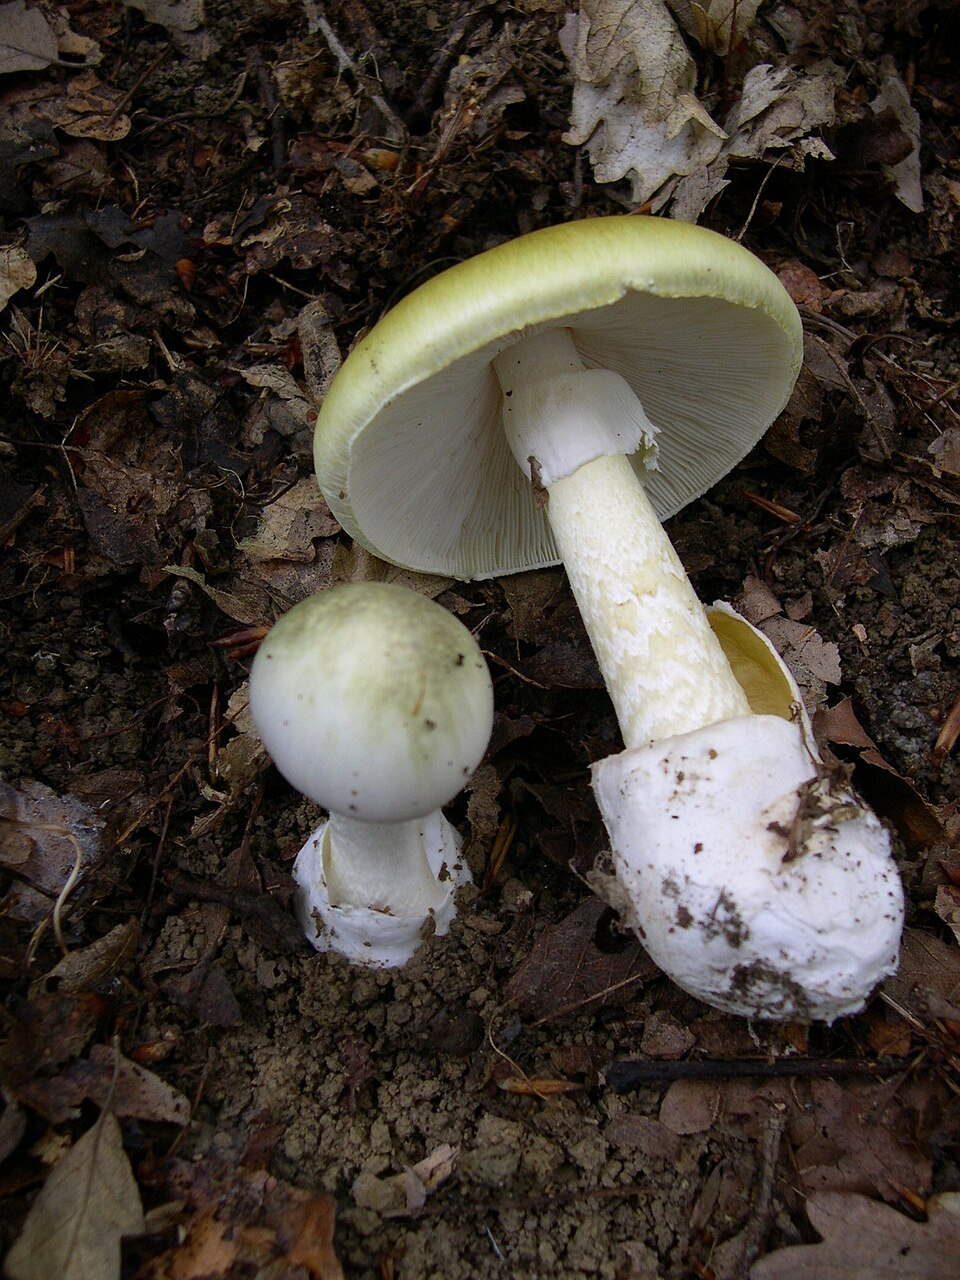
\includegraphics[width=0.3\columnwidth]
    {Amanita_phalloides_1.JPG}};
\node[below=0.05cm of inputimg, 
      font=\small\itshape] (inputlabel) 
    {Amanita phalloides};

% Stage 1
\node[box, fill=blue!10, 
      below=0.3cm of inputlabel] (s1){
    \textbf{Stage 1 Vision API}\\
    \footnotesize YOLOv26n-cls $\cdot$ TFLite float16};

% Stage 2
\node[box, fill=green!10, 
      below=0.3cm of s1] (s2){
    \textbf{Stage 2 Ecological Retrieval}\\
    \footnotesize mushroom\_context.json};

% Stage 3
\node[box, fill=orange!10, 
      below=0.3cm of s2] (s3){
    \textbf{Stage 3 LLM Audit}\\
    \footnotesize Gemini Flash Lite};

% Stage 4
\node[box, fill=red!10, 
      below=0.3cm of s3] (s4){
    \textbf{Stage 4 Risk Classifier}\\
    \footnotesize Rule-based Python};

% Output screenshot
\node[below=0.3cm of s4] (outputimg){
    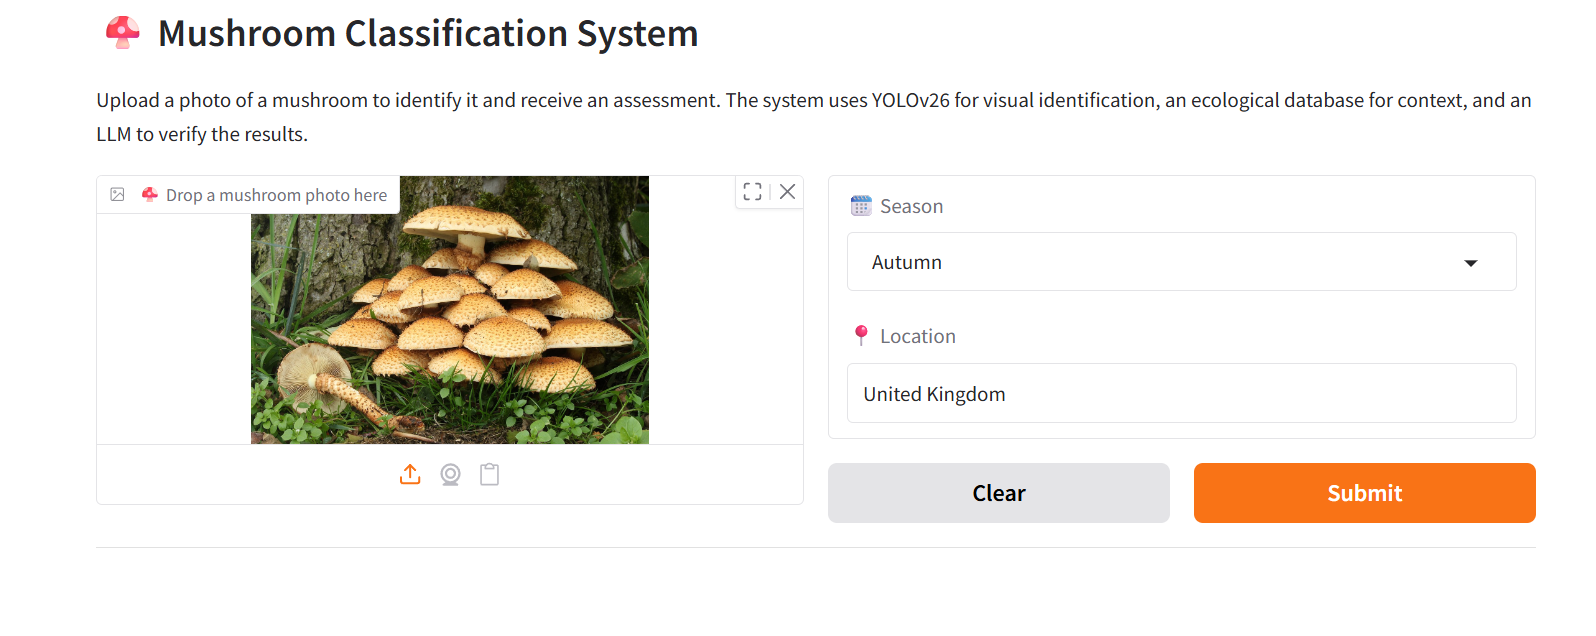
\includegraphics[width=0.9\columnwidth]
    {Gradio_UI.png}};
\node[below=0.05cm of outputimg,
      font=\small\itshape] (outputlabel)
    {Structured report in Gradio interface};

% Arrows with labels
\draw[arrow] (inputlabel) -- 
    node[label, right]{image} (s1);
\draw[arrow] (s1) -- 
    node[label, right]{species + confidence} (s2);
\draw[arrow] (s2) -- 
    node[label, right]{12-field record} (s3);
\draw[arrow] (s3) -- 
    node[label, right]{verdict + reasoning} (s4);
\draw[arrow] (s4) -- 
    node[label, right]{risk level} (outputimg);

\end{tikzpicture}
\caption{End-to-end pipeline for 
\textit{Amanita phalloides}: input image (top), 
four-stage processing (middle), and structured 
Gradio output (bottom).}
\label{fig:pipeline-full}
\end{figure}


 
% ============== RESULTS AND ANALYSIS 
\section{\textbf{Results and Analysis}}
 
This section presents the experimental results in relation to the research questions. First, compares the three selected vision architectures on the internal 169 species test set to evaluate the trade off between classification and deployment efficiently. Second, YOLOv26n-cls is evaluated on the external DF24-Mini benchmark to assess generalization beyond the primary dataset. Third, an ablation study compares vision only, standalone Gemini baseline and multimodal configurations to measures the contribution of the LLM audit layer to safety-oriented decision suppor. Finally, the structured application output is compared with a standard unimodal classifier output to assess whether the proposed system provides more interpretable information than a standard image classification.
 

\subsection{\textbf{Internal Baseline Vision Model Benchmarking}}\label{subsec:baseline}
 
Table~\ref{tab:main-leaderboard} compares the three selected vision models on the held-out 10\% test split of the 169 species mushroom dataset, and Fig. ~\ref{fig:validation-accuracy-trends} shows the Top-1 and Top-5 accuracy trends across training epochs. The purpose of this experiment was to evaluate which model provided the best balance between classification performance and deployment efficiently. 

DINOv2-Small achieved the highest Top-1 accuracy at 92.4\%, indicating that self-supervised vision transformer features were effective for fine gain mushroom classification. ConvNeXt-Tiny also performed strongly with Top-1 accuracy at 91.1\%. However these improvement required substantially larger deployment resources. Dinov2-Small used 22.0M parameters and an 85 MB model file and ConvNeXt-Tiny contained 28.6 Parameters and produced a 110 MB model file.

YOLOv26n-cls achieved a lower Top-1 accuracy of 88.1\%, but reach 98.4\% Top-5 accuracy matching the strongest Top-5 performance among the benchmarked models. 

Although YOLOv26n-cls Top-1 accuracy was lower than  DINOv2-Small and ConvNeXt-Tiny, its Top-5 accuracy were nearly identical to the larger models. This means that YOLOv26n-cls often included the correct species among its top predictions, even when the first prediction was not always correct. 

In addition, after conversion to TFLite float16, YOLOv26n-cls was also much smaller and faster than the large models, with only 1.74M parameters and produced a 3.6 MB model file and CPU inference time at 4.8 ms. Fig.~\ref{fig:model-comparison} provides an illustrative single image comparison using an Amanta phalloidas test image. All three models predict the correct 
species while YOLOv26n-cls achieved the fastest 
inference time at 3.8ms and fewest parameters 1.74M in this example. However, this figured is used as a qulaitative illustration; the deployment decision is primary supported bu the full benchmark results in Table~\ref{tab:main-leaderboard}.

Therefore, YOLOv26n-cls was selected as the deployment model because it provided the best trade-off between classification performance, model size, inference speed, and deployment practicality. 

The full six model benchmark, including
EfficientNet-B0, YOLOv8n-cls, YOLOv11n-cls,is reported in Appendix~\ref{app:full-bench}, Table~\ref{tab:full-leaderboard}.


\begin{figure}[h]
\centering
\begin{tikzpicture}
    \node[anchor=south west, inner sep=0] (image) at (0,0)
        {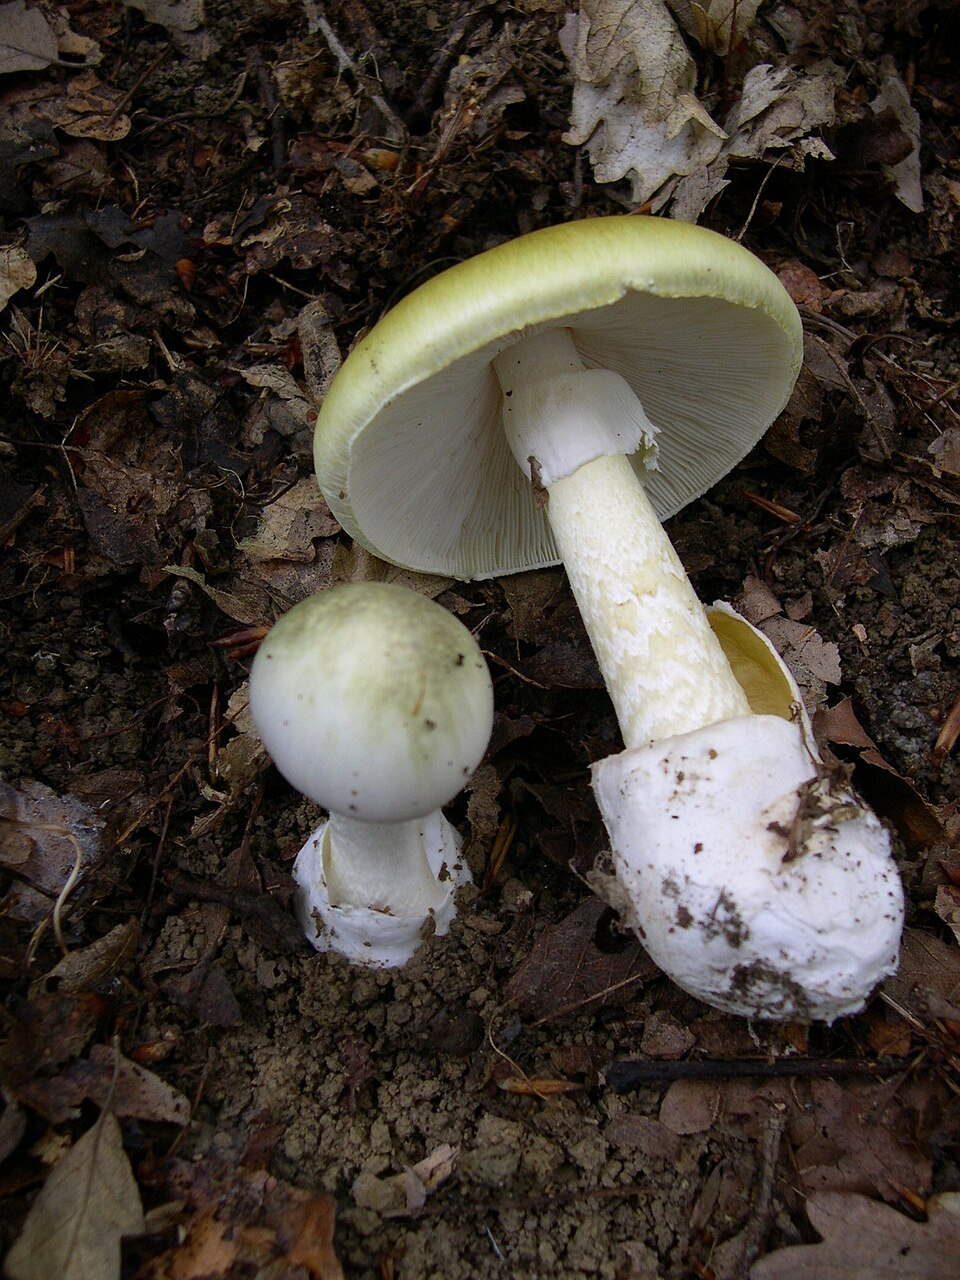
\includegraphics[width=0.55\columnwidth]
        {Amanita_phalloides_1.JPG}};
    
    \begin{scope}[x={(image.south east)},
                  y={(image.north west)}]
        
        % ConvNeXt label — grey
        \node[fill=gray!80!black, fill opacity=0.85, 
              text opacity=1, text=white, 
              font=\footnotesize\bfseries,
              rounded corners=3pt, 
              inner sep=4pt,
              anchor=north west] 
              at (0.02, 0.98) 
              {ConvNeXt-Tiny \quad 71.4\% \quad 
              6.6ms \quad 27.95M};
        
        % DINOv2 label — blue
        \node[fill=blue!60!black, fill opacity=0.85,
              text opacity=1, text=white,
              font=\footnotesize\bfseries,
              rounded corners=3pt, 
              inner sep=4pt,
              anchor=north west]
              at (0.02, 0.91)
              {DINOv2-Small \quad 89.1\% \quad 
              7.8ms \quad 22.12M};
        
        % YOLO label — green
        \node[fill=green!50!black, fill opacity=0.85,
              text opacity=1, text=white,
              font=\footnotesize\bfseries,
              rounded corners=3pt, 
              inner sep=4pt,
              anchor=north west]
              at (0.02, 0.84)
              {YOLOv26n-cls \quad 95.5\% \quad 
              3.8ms \quad 1.74M \checkmark};

        % Species label at bottom
        \node[fill=black, fill opacity=0.75,
              text opacity=1, text=white,
              font=\footnotesize\itshape,
              rounded corners=3pt, 
              inner sep=4pt,
              anchor=south west]
              at (0.02, 0.02)
              {Amanita phalloides --- Ground Truth};
              
    \end{scope}
\end{tikzpicture}
\caption{Confidence scores, CPU latency, and parameter count overlaid on the same 
\textit{Amanita phalloides} test image.}
\label{fig:model-comparison}  % ← must be HERE
\end{figure}


\begin{table}[t]
\centering
\caption{Comparison of the three benchmarked architectures}
\label{tab:main-leaderboard}
\small
\renewcommand{\arraystretch}{1.25}
\setlength{\tabcolsep}{2.8pt}
\begin{tabular}{lccccc}
\hline
\textbf{Model} & \textbf{Top-1} & \textbf{Top-5} & \textbf{Params} & \textbf{Size} & \textbf{CPU} \\
\noalign{\hrule height 0.9pt}
ConvNeXt-Tiny        & 91.1 & 98.3 & 28.6M & 110 MB & 35.6ms \\
DINOv2-Small         & \textbf{92.4} & \textbf{98.4} & 22.0M & 85 MB & 32.2ms \\
YOLOv26n-cls f16     & 88.1 & \textbf{98.4} & \textbf{1.74M} & \textbf{3.6 MB} & \textbf{4.8ms} \\
\hline
\multicolumn{6}{l}{\footnotesize *CPU latency for DINOv2-Small was not measured.} \\
\end{tabular}
\end{table}


\begin{figure}[t]
    \centering
    \includegraphics[width=\linewidth]{Top1andTop5Accuracy.png}
    \caption{Top-1 and Top-5 accuracy trends.}
    \label{fig:validation-accuracy-trends}
\end{figure}
 
 
\subsection{\textbf{External Benchmark: DF24-Mini (RQ1)}}\label{subsec:df24}
 
Table~\ref{tab:df24-main} compares YOLOv26n-cls with published DF24-Mini benchmark baselines. We aim to evaluate whether the selected deployment architecture could remain competitive on an external fungi classification benchmark.
 
\begin{table}[h]
\centering
\caption{DF24-Mini benchmark results. Baselines are from
Picek et al.~\cite{picek2022danishfungi}; our result was evaluated at epoch~37.}
\label{tab:df24-main}

\small
\setlength{\tabcolsep}{4pt}
\renewcommand{\arraystretch}{1.12}

\begin{tabular}{@{}lccc@{}}
\hline
\textbf{Model} & \textbf{Params} & \textbf{Top-1} & \textbf{Top-3} \\
\hline
ViT-Large/16                 & 307M  & 67.52\% & 84.46\% \\
ViT-Base/16                  & 86M   & 65.33\% & 82.44\% \\
SE-ResNeXt-101               & 49M   & 62.42\% & 80.71\% \\
\textbf{YOLOv26n-cls (Ours)} & \textbf{1.74M} & \textbf{60.17\%} & \textbf{78.93\%} \\
EfficientNet-B3              & 12M   & 59.31\% & 78.79\% \\
EfficientNet-B0              & 5.3M  & 58.58\% & 77.01\% \\
\hline
\multicolumn{4}{@{}p{0.95\linewidth}@{}}{
\footnotesize *The DF24-Mini benchmark was performed only on YOLOv26n-cls. Therefore, external benchmarking of ConvNeXt-Tiny and DINOv2-Small is left for future work.
} \\
\end{tabular}
\end{table}
 
YOLOv26n-cls achieved stronger Top-1 and Top-3 performance than both EfficientNet baselines, regardless of using much smaller parameters budget. However, it remained below the larger ViT-Large, ViT-Base, and SE-ResNeXt-101 models, which is expected because those models have substantially higher parameter budgets. 

Therefore, the external benchmaek does not show that YOLOv26n-cls is the most accurate model overall. Instead, it supports its suitability as a lightweight deployment model that remain competitive, while requiring  uch smaller parameters than the highest performing published baselines.  

Overall, the DF24-Mini result strengthens the main finding from the internal benchmark. Its provides a practical trade off between accuracy and  deployment cost, making YOLOv26n-cls suitable for the final multimodal pipeline.

 
\subsection{\textbf{Ablation Study: Unimodal vs Multimodal}}\label{subsec:ablation}

Table \ref{tab:ablation_full_results} compares three types of configurations: unimodal visual baseline, standalone Gemini baseline and multimodal vision with Gemini pipelines. 

\begin{table}[h!]
\centering
\caption{Ablation study on 300 images: 203 dangerous cases and 97 safe cases.}
\label{tab:ablation_full_results}

\small
\setlength{\tabcolsep}{4pt}
\renewcommand{\arraystretch}{1.15}

\begin{tabular}{@{}lccc@{}}
\hline
\textbf{Configuration} & \textbf{Safety Recall} & \textbf{FPR} & \textbf{F1 Score} \\
\hline
YOLOv26n *standalone         & 30.0\% & 16.5\% & 44.2\% \\
DINOv2-S *standalone          & 15.3\% & \textbf{0.0\%}  & 26.5\% \\
ConvNeXt-T *standalone        & 14.3\% & \textbf{0.0\%}  & 25.0\% \\
\hline
Gemini LLM Only       & \textbf{92.6\%} & 70.7\% & 81.6\% \\
\hline
YOLOv26n-Gemini *(15.3ms)      & 75.9\% & 18.6\% & 80.0\% \\
ConvNeXt-T-Gemini *(30.1ms)    & 73.4\% & 10.3\% & 81.2\% \\
DINOv2-S-Gemini *(38.7ms)      & 74.9\% & 10.3\% & \textbf{81.9\%} \\
\hline
\multicolumn{4}{@{}p{0.95\columnwidth}@{}}{
\footnotesize *FPR = false positive rate, meaning the percentage of safe images incorrectly flagged as dangerous.
} \\
\end{tabular}
\end{table}

\textbf{(1) Unimodal vision baseline result.} The results demonstrate that using only vision classification baseline was not sufficient for safety critical mushroom identification. YOLOv26n-cls detected 30.0\% of dangerous cases, while ConvNeXt-Tiny and DINOv2-Small detected only 14.3\% and 15.3\%, respectively. This means that the vision classification baseline system missed most classification between 70.0\% and 85.7\% of dangerous cases. In addition, the 0.0\% false positive rate for DINOv2-Small and ConvNeXt-Tiny shows that these models did not incorrectly flag safe mushroom as dangerous. However, this low false positive rate came at the cost of very low safety recall, meaning that they also failed to flag most dangerous mushrooms. Although ConvNeXt-Tiny and DINOv2-Small achieved higher classification accuracy in the internal benchmark, this did not translate into better safety recall in the fallback setting. This means that classification accuracy alone is not sufficient for evaluating a safety-oriented mushroom identification system. 


\textbf{(2) Standalone Gemini baseline result.} Standalone Gemini baseline achieved a highest safety recall at 92.6\%, meaning that it detected most dangerous mushroom cases. However, it also incorrectly flagged 70.7\% of safe cases as dangerous. This high false positive rate shows that Gemini was too conservative and impractical as a standalone baseline in this study. In practical use, this means that the model would flags almost every mushroom, including common edible ones as a dangerous species.

% This excessive false classification may reduce user trust in the system.

\textbf{(3) Multimodal result.}
The multimodal configurations provided a better balance between classify dangerous mushrooms and avoiding the excessive false detection. YOLOv26n-cls with Gemini achieved 75.9\% safety recall and an F1 score of 80.0\%. ConvNeXt-Tiny with Gemini and DINOv2-Small with Gemini achieved slightly higher F1 scores of 81.2\% and 81.9\%, respectively. The Gemini audit layer reduced the performance gap between the lightweight YOLOv26n-cls model and the larger vision models.

\textbf{(4) Deployment decision.}
Therefore, the final modal choice was guided by deployment practically rather than focusing solely on the classification accuracy alone. Although, DINOv2-Small with Gemini achieved the highest F1 score, YOLOv26n-cls wth Gemini provided a comparable safety result with a much smaller modal size and fastest speed inference. In the ablation harness, for speed inference during the real time classification, YOLOv26n-cls required only 15.3 ms per image compared with 30.1 ms for ConvNeXt-Tiny and 38.7 ms for DINOv2-Small. Since the Gemini API call already slower the overall pipeline latency, the difference between the vision modesl has less impact on the final user facing response time. Therefore YOLOv26n-cls was selected as the most practical deployment because it provides the best balance between safety performance, inference speed, model size, and deployment feasibility.



 
\subsection{\textbf{Comparison of Unimodal and  Multimodal Outputs}}

To address RQ4, we compares the output produced by (a)~a standard unimodal classifier with (b)~the structured output from the proposed multimodal pipeline using YOLOv26n-cls as the vision modal and Gemini as the interpreability. The classification accuracy of these two scenario is evaluated on section C, in this section we focused on the final application output. 

The pipeline's structured report contains 13 fields including identification, ecological grounding, and risk reasoning, retrieved from the ecological database
(\texttt{mushroom\_context.json} section~\ref{sec:ecological-db}. Table~\ref{tab:output-comparison} illustrates this using
\textit{Amanita phalloides} image. A YOLOv26n-cls unimodal system returns only a predicted species name and confidence score of 0.96, providing insufficient data for user. In contrast, the multimodal pipeline additionally returns toxicity class, edibility, habitat, season, geographic region, known lookalikes, key warnings, LLM reasoning, risk level, and a plain-language recommendation. The example at Fig.~\ref{fig:amanita} shows the corresponding live application output and demonstrating how the structured output is presented in the Gradio interface. 

\begin{table}[h!]
\centering
\caption{Output comparison for a single \textit{Amanita phalloides}
         image: unimodal classifier versus the multimodal pipeline.}
\label{tab:output-comparison}
\normalsize
\begin{tabular}{p{2.1cm} p{1.6cm} p{4.2cm}}
\hline
\textbf{Field} & \textbf{Unimodal} & \textbf{Multimodal pipeline} \\
\hline
Predicted species  & \textit{A.phalloides} & \textit{Amanita phalloides}                      \\[3pt]
Confidence         & 0.96                   & 0.96                                             \\[3pt]
Toxicity class     & x                     & Deadly                                           \\[3pt]
Edibility          & x                     & Fatally poisonous                                \\[3pt]
Habitat            & x                     & Deciduous woodland                               \\[3pt]
Active season      & x                     & Summer-Autumn                                   \\[3pt]
Region             & x                     & Europe, North America                            \\[3pt]
Lookalikes         & x                     & \textit{A.~citrina}, \textit{V.~volvacea}        \\[3pt]
Key warnings       & x                     & Amatoxins; symptoms delayed 6--24\,h             \\[3pt]
LLM verdict        & x                     & DANGER - volva and gills consistent with
                                                   \textit{A.~phalloides}                         \\[3pt]
Risk level         & x                     & \textbf{CRITICAL}                                \\[3pt]
Recommendation     & x                     & Do not consume. Seek medical advice if ingested. \\
\hline
\textbf{Total}     & \textbf{2}             & \textbf{13}                                      \\
\hline
\end{tabular}
\end{table}
  
% -----------------
% FIGURE: App screenshot (swap in your real image)
% -----------------

% Mushroom image paired with the comparison table
\begin{figure}[h]
    \centering
    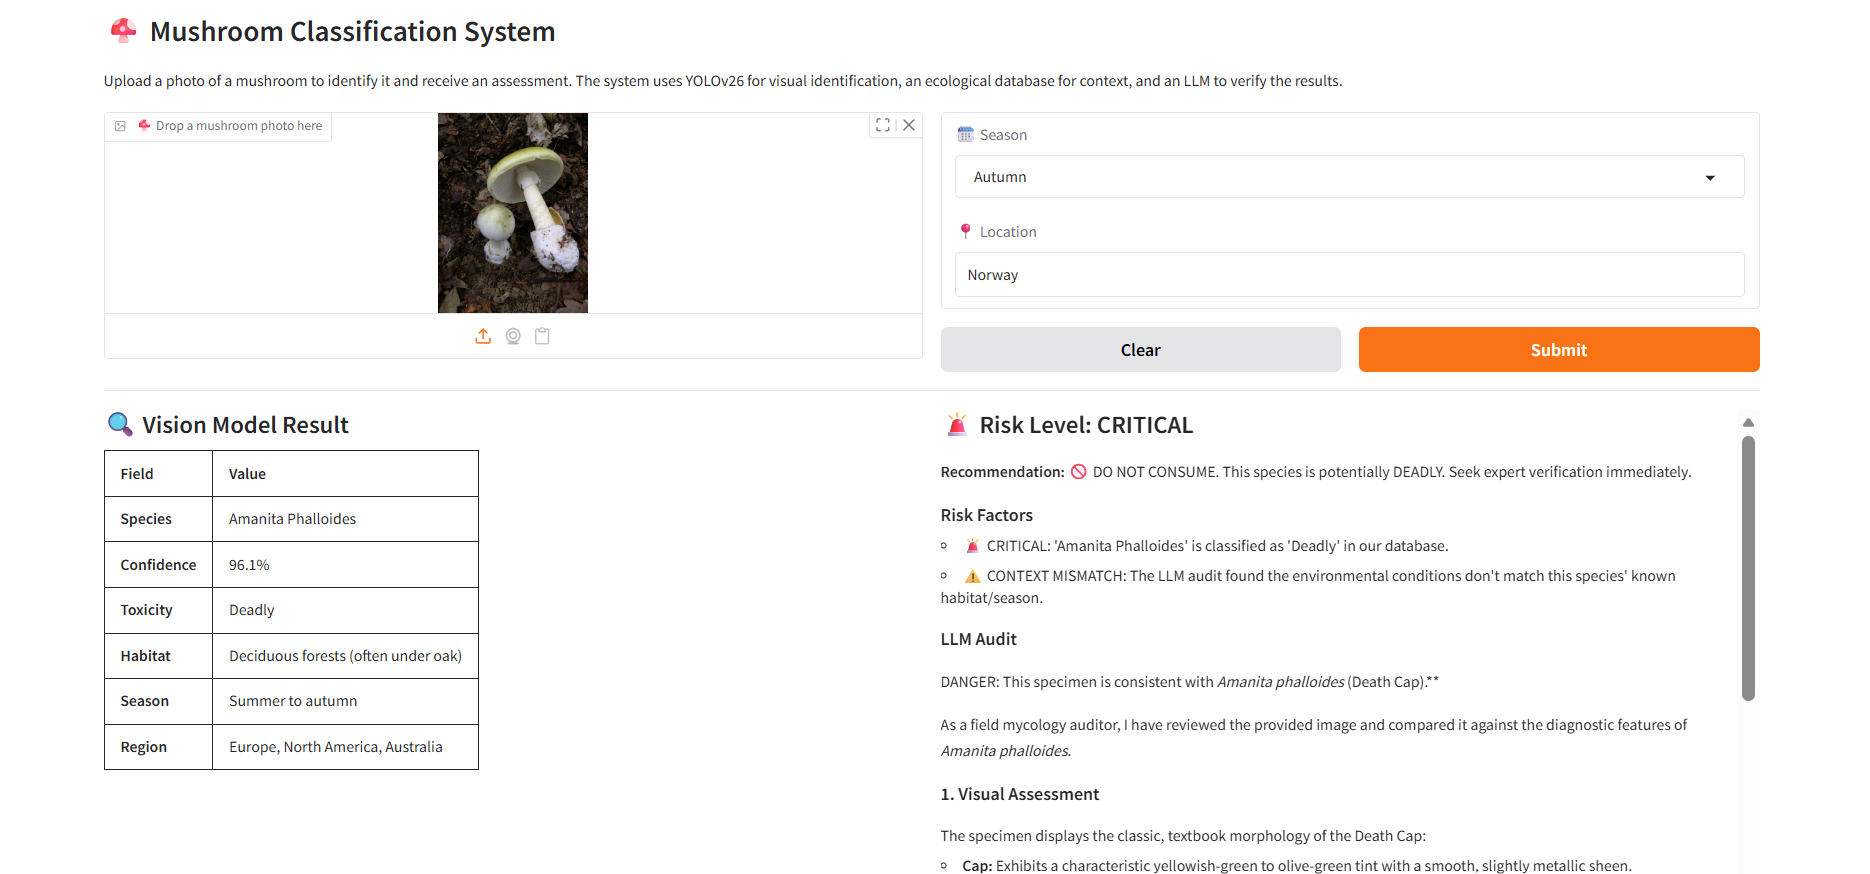
\includegraphics[width=1\linewidth]{AmanitaPhalloides.png}
    \caption{Live pipeline output for \textit{Amanita phalloides},
             showing the \textbf{CRITICAL} risk verdict, LLM audit,
             and plain-language recommendation from
             Table~\ref{tab:output-comparison} rendered in the
             Gradio interface. Ecological fields are sourced from
             \texttt{mushroom\_context.json} and do not replace
             expert mycological identification.}
    \label{fig:amanita}
\end{figure}

Overall, this comparison shows that the proposed pipeline improves interpreability by transforming a raw classification score into a structured safety report with ecological grounding, risk interpretation and user oriented guidance. The output does not replace expert mycological identification, but it provides more meaningful decision support information for non technical users than a standalone image classier. 




% ------ Discussion ------
\section{\textbf{Discussion}}

These results shows that neither image classification alone nor standard Gemini was sufficient for reliable edible and toxic assessment. The image-only identification model missed classify between 70.0\% and 85.7\% of dangerous cases. In contrast, Gemini detects most dangerous cases but incorrectly flagged 70.7\% of safe cases as dangerous. DINOv2-Small and ConvNeXt-Tiny achieved higher Top-1 accuracy than YOLOv26n-cls in the internal benchmarking but they performed worse in the ablation setting. 

A key finding is that higher species classification accuracy did not lead to better toxic-risk detection, because the vision models were trained to classify species, not to directly reason about edibility or toxicity. In the vision-only setting, the 70\% threshold acted only as an uncertainty warning, not as true toxicity reasoning. This highlights the importance of adding ecological context and an LLM audit layer. This indicate that a single component system is not suitable at detecting toxic risk and too conservative for practical use. 

The multimodal provided the best balance, with F1 score between 80.0\% and 81.9\%. When Gemini was added, all three multimodal configurations achieved very similar F1 scores, between 80.0\% to 81.9\%  This findings support the main decision to combine vision classification with ecological metadata and an Gemini LLM audit layer.


The results from the external DF24-Mini benchmark further support the deployment selection. YOLOv26n-cls did not achieve the highest accuracy overall, but it remained competitive against published baselines that requiring far fewer parameters than a large ViT and SE-ResNeXt models. In addition, YOLOv26n-cls also required only 15.3 ms per image in the ablation harness, compared with 30.1 ms for ConvNeXt-Tiny and 38.7 ms for DINOv2-Small. 

These results supports the deployment selection of YOLOv26n-cls, since the prior efficient deep learning research emphasizes that deployed vision models should be evaluated not only by accurcay, but also by latency, model size, and computational effiiceny.  Therefore,  YOLOv26n-cls was selected becuase its provides the best practical trade-off between classification performance inference speed, model size, and deployment feasibility \cite{howard2017mobilenets}. 

The structure output comparison addresses RQ3 by further analysis that the proposed pipeline provides more useful information than a standard vision classifier. A vision model only returns a species label and confidence score which is provides no basic knowledge to evaluate whether to trust the prediction or what action should be taken. In contrast, the propose multimodal model generates a 12 field report that includes toxicity class, ecological context, risk level, LLM reasoning, and user guidance. This design support the main aim of the study that to build a mushroom identification system that is more interpretable and more useful.
 
\textbf{Limitations:} However, we aware that our research may have several limitations due to the time constraint of the project and the safety critical. First, the ecological database was developed as a prototype knowledge base, compile from open-source resources, and the database was not validated by expert mycologist. 

Second, the system was not evaluated with real users, so the structure output has not yet been tested in real word contexts. Therefore, the system should be understood as a decision support prototype rather than a replacement for expert mushroom identification. 

\textbf{Future Work:} Future work should include the large scale of validation, expert review of the ecological database and testing on the user in order to evaluate whether the structured output is useful and understandable in real world contexts.

In additin, the researahc can pocus more of the experiment that centerd around the trad off between latency and accurcay in real word production becuase not some fields for exaple in medical data reqires more accyracy than latency and filed like financal that requires fast than accurcay. 




% ------ Conclusion------
\section{\textbf{Conclusion}}

This study proposed a unified multimodal mushroom classification framework that combines vision-based species classification, ecological context retrieval, Gemini-based LLM auditing, and structured output generation. The results show that image classification alone is not sufficient for reliable edible and toxic assessment, because vision models mainly predict species labels and do not directly reason about toxicity or ecological risk.

Across the experiments, YOLOv26n-cls was selected as the final deployment model because it provided the best practical trade-off between classification performance, model size, inference speed, and deployment feasibility. Although larger models achieved higher Top-1 accuracy, their advantage became less important once the Gemini audit layer was added.

The ablation study showed that the multimodal pipeline provided a better balance than either vision-only classification or Gemini alone. In addition, the structured output comparison showed that the proposed system provides more useful information than a standard classifier by adding toxicity, ecological context, risk level, LLM reasoning, and user guidance.

The system remains a prototype. The ecological database requires expert validation, and user testing in real foraging conditions has not yet been conducted. These are the most important directions for future work before the system could be considered for broader deployment.

Overall, this study demonstrates that safety-oriented mushroom identification benefits from integrating vision, ecological knowledge, and language reasoning into a unified pipeline, and that this integration is achievable within practical deployment constraints.

\bibliographystyle{IEEEtran}
\bibliography{references}



 

% if have a single appendix:
%\appendix[Proof of the Zonklar Equations]
% or
%\appendix  % for no appendix heading
% do not use \section anymore after \appendix, only \section*
% is possibly needed

% use appendices with more than one appendix
% then use \section to start each appendix
% you must declare a \section before using any
% \subsection or using \label (\appendices by itself
% starts a section numbered zero.)
%

\clearpage
\appendices

\section{\textbf{Full Architecture Benchmark}}\label{app:full-bench}


This appendix reports the full eight-architecture exploration referenced in Section~\ref{subsec:baseline} The main results section reports only the three selected models, however the wider experiment included additional baselines to support the final model selection decision. 

The selected models represent different architecture families: YOLOv26n-cls as a lightweight deployment-oriented classifier, ConvNeXt-Tiny as a modern CNN baseline, and DINOv2-Small as a self-supervised Vision Transformer. Additional models, including EfficientNet-B0, YOLOv8n-cls, and TaxonomicYOLO26, were included as secondary baselines.
 
Table~\ref{tab:full-leaderboard} reports every trained model on the held-out 10\% test split of the 169 species dataset. Accuracy values are therefore directly comparable and the model were trained locally on an RTX4070.

The full shows that DINOv2-Small achieved the highest Top-1 accuracy, while ConvNeXt-Tiny also performed strongly. YOLOv26n-cls achieved lower Top-1 accuracy, but remained competitive in Top-5 accuracy and had the smallest deployment footprint after TFLite float16 export. This appendix therefore provides the detailed evidence behind the deployment trade-off discussed in the main results section.


 
\begin{table*}[!t]
\centering
\caption{ Across all trained architectures on the
169-species held-out test split (80/10/10, batch=1, 224$\times$224).}
\label{tab:full-leaderboard}
\small
\begin{tabular}{@{}lccrrrrl@{}}
\hline
\textbf{Model} & \textbf{Top-1} & \textbf{Top-5} & \textbf{Params}
& \textbf{Size} & \textbf{GPU (ms)} & \textbf{CPU (ms)} & \textbf{Notes} \\
\hline
DINOv2-Small               & 92.8\%          & 98.4\%          & 22.0M & 85 MB    & 10.2   & 32.2   & Self-supervised ViT, accuracy leader \\
ConvNeXt-Tiny (PEFT)       & 91.1\%          & 98.3\%          & 28.6M & 110 MB   & 7.6  & 35.6 & Modern CNN, PEFT two-phase           \\
EfficientNet-B0            & 89.5\%          & 97.9\%          & 5.3M  & 17.2 MB  & 11.6 & 19.2 & Classification-native CNN            \\
YOLOv26n-cls (PyTorch)     & 88.1\%          & 98.4\%          & 1.74M & 3.6 MB   & 6.3  & 7.1  & Production source                    \\
YOLOv26n-cls (TFLite f16)  & 88.1\%          & 98.4\%          & 1.74M & 3.6 MB   & 3.8   & 4.8  & \textbf{Deployed model}              \\
YOLOv8n-cls                & 86.8\%          & 97.9\%          & 2.7M  & 3.4 MB   & 4.6  & 6.3  & Original baseline                    \\
YOLOv11n-cls               & 87.66\%          & 98.11\%          & 2.7M  & 3.4 MB   & 4.6  & 6.3  & Original baseline                            \\
\hline
\multicolumn{8}{l}{\textit{Scoped but not trained:}~ViT-S/16 and TaxonomicYOLO26} \\
\hline
\end{tabular}
\end{table*}
 
\section{\textbf{Ecological Database Schema}}
\label{app:eco-schema}

This appendix describes the structure of the ecological database used in the multimodal pipeline. The database was implemented as a JSON file containing one record for each of the 169 mushroom species included in the system. Each entry contains 12 fields per species as defined 
in Table~\ref{tab:eco-schema}. The JSON descriptions
illustrates two example entries using an edible and toxic 
lookalike pair, demonstrating how the database supports 
species disambiguation in the LLM audit layer.

\begin{table}[h]
\centering
\normalsize
\caption{Ecological database field definitions (12 fields per species entry).}
\label{tab:eco-schema}
\begin{tabular}{ll}
\hline
\textbf{Field} & \textbf{Description} \\
\hline
species\_name     & Scientific species name \\
toxicity\_type    & Edible, Toxic, Deadly, or Hallucinogenic \\
habitat           & Typical growth environment \\
season            & Active fruiting period \\
region            & Geographic distribution \\
key\_warnings     & Safety-critical identification notes \\
cap\_description  & Morphological cap features \\
gill\_description & Gill colour, structure, and spacing \\
stem\_description & Stem height, colour, and ring presence \\
smell             & Characteristic odour \\
lookalikes        & Similar species with key differences \\
environment\_tips & Contextual foraging guidance \\
\hline
\end{tabular}
\end{table}

\begin{figure}[h]
\footnotesize
\begin{verbatim}
[
  {
    "species_name": "Agaricus augustus",
    "toxicity_type": "Edible",
    "habitat": "Coniferous and mixed forests",
    "season": "Late summer to autumn",
    "region": "North America, Europe",
    "key_warnings": "Beware yellow staining at base.",
    "cap_description": "Large (10-25cm), brown scales.",
    "gill_description": "White to chocolate brown.",
    "stem_description": "Tall (10-20cm), ring present.",
    "smell": "Strongly of anise or almonds.",
    "lookalikes": "A. xanthodermus (yellow, phenol).",
    "environment_tips": "Near spruce or pine."
  },
  {
    "species_name": "Agaricus xanthodermus",
    "toxicity_type": "Toxic",
    "habitat": "Grassy areas, gardens, parks",
    "season": "Late summer to autumn",
    "region": "North America, Europe, Australia",
    "key_warnings": "Stains bright yellow when bruised.",
    "cap_description": "Medium (5-15cm), stains yellow.",
    "gill_description": "Pinkish-grey, never white.",
    "stem_description": "Bulbous base, yellow when cut.",
    "smell": "Ink, phenol, or library paste.",
    "lookalikes": "A. arvensis (slow yellow, anise).",
    "environment_tips": "Lawns, compost heaps after rain."
  }
]
\end{verbatim}
\caption{Example records from \texttt{mushroom\_context.json}}
\label{fig:eco-example}
\end{figure}

The ecological database was used by the pipeline in two ways. First, it supplied structured context to the LLM audit prompt. Second, it supplied user-facing information in the final structured output, including toxicity, habitat, lookalikes, warnings, and recommendation fields.

\textit{Note: The database should be interpreted as a prototype knowledge base. The records were compiled from open online sources and were not independently validated by a professional mycologist. Future work should include expert review and correction of the ecological records before the system is used in real-world foraging contexts.}

 

\section{\textbf{Ablation Test Set: Dangerous Species}}
This appendix provides additional details for the ablation study reported in Section IV-C. The purpose of the ablation study was to evaluate how much each system component contributed to edible/toxic risk assessment when tested in isolation and in combination

The ablation evaluation was restricted to the 40 species below, selected from the held-out test split (\texttt{data/dataset\_split/test/}) on the basis that their toxicity classification contains at least one of the following keywords: Deadly, Highly Toxic, Toxic, Hallucinogenic, or Pathogenic. Up to 20 images per species were sampled (seed 42), yielding a maximum of 800 images. Table~\ref{tab:app_c_species} lists all 40 species included in the evaluation.


\begin{table*}[h]
\centering
\caption{Ablation Study Test Set: 40 Dangerous Species}
\label{tab:app_c_species}
\normalsize
\begin{tabular}{@{}llll@{}}
\hline
\textbf{Species} & \textbf{Toxicity} & \textbf{Species} & \textbf{Toxicity} \\
\hline
\textit{Amanita phalloides} & Deadly & \textit{Pholiota squarrosa} & Toxic \\
\textit{Galerina marginata} & Deadly & \textit{Stropharia aeruginosa} & Edible (C) / Toxic \\
\textit{Paxillus involutus} & Deadly & \textit{Clitocybe nebularis} & Toxic (For many) \\
\textit{Gyromitra esculenta} & Deadly (Raw)/Toxic & \textit{Coprinopsis atramentaria} & Toxic (w/ alcohol) \\
\textit{Amanita pantherina} & Highly Toxic & \textit{Hygrophoropsis aurantiaca} & Toxic (Mild)/Edible \\
\textit{Agaricus xanthodermus} & Toxic & \textit{Lactarius torminosus} & Toxic (R)/Edible (P) \\
\textit{Amanita augusta} & Toxic & \textit{Panaeolus papilionaceus} & Toxic (Mild) \\
\textit{Amanita brunnescens} & Toxic & \textit{Schizophyllum commune} & Toxic / Pathogenic \\
\textit{Amanita citrina} & Toxic & \textit{Tapinella atrotomentosa} & Toxic (R)/Edible (P) \\
\textit{Amanita flavoconia} & Toxic & \textit{Verpa bohemica} & Toxic (R)/Edible (P) \\
\textit{Chlorophyllum brunneum} & Toxic & \textit{Vulpicida pinastri} & Toxic (Lichen) \\
\textit{Chlorophyllum molybdites} & Toxic & \textit{Amanita muscaria} & Toxic / Halluc. \\
\textit{Gyromitra gigas} & Toxic & \textit{Amanita persicina} & Toxic / Halluc. \\
\textit{Gyromitra infula} & Toxic & \textit{Gymnopilus luteofolius} & Toxic / Halluc. \\
\textit{Hypholoma fasciculare} & Toxic & \textit{Psilocybe azurescens} & Toxic / Halluc. \\
\textit{Lactarius turpis} & Toxic & \textit{Psilocybe caerulescens} & Toxic / Halluc. \\
\textit{Leratiomyces ceres} & Toxic & \textit{Psilocybe cubensis} & Toxic / Halluc. \\
\textit{Omphalotus illudens} & Toxic & \textit{Psilocybe cyanescens} & Toxic / Halluc. \\
\textit{Omphalotus olivascens} & Toxic & \textit{Psilocybe ovoideocystidiata} & Toxic / Halluc. \\
\textit{Pholiota aurivella} & Edible (C) / Toxic & \textit{Psilocybe pelliculosa} & Toxic / Halluc. \\
\hline
\end{tabular}%
\end{table*}






\section{\textbf{LLM Audit System Prompt (Ollama/Gemini})}
\label{app:llm-prompt}

The following prompt was submitted to Gemini Flash Lite at Stage 3 of the pipeline for each input image during both ablation evaluation and production deployment.

The following prompt was used for the LLM audit layer alongside each mushroom photograph during evaluation.

\textbf{System Prompt:} You are a field mycology safety auditor. You have been given a photo of a mushroom taken in the field. A computer vision model identified it as [PREDICTED SPECIES] with [CONFIDENCE]\% confidence.

Ecological database entry for [PREDICTED SPECIES]:
\begin{itemize}
    \item Toxicity: [TOXICITY]
    \item Edibility: [EDIBILITY]
    \item Typical habitat: [HABITAT]
    \item Season: [SEASON]
    \item Region: [REGION]
    \item Key warnings: [KEY WARNINGS]
\end{itemize}

Visual identification features to check in the photo:
\begin{itemize}
    \item Cap: [CAP DESCRIPTION]
    \item Gills: [GILL DESCRIPTION]
    \item Stem: [STEM DESCRIPTION]
    \item Smell: [SMELL]
    \item Dangerous lookalikes: [LOOKALIKES]
\end{itemize}

Your Task:
\begin{enumerate}
    \item Look at the photo carefully and compare it against the known features above.
    \item Comment on what you can see - cap shape/colour, gill colour, stem, any bruising or staining.
    \item Mention relevant field checks the user should do in person.
    \item State AGREE if the photo is consistent with [PREDICTED SPECIES], or DISAGREE if something looks wrong.
    \item If the species is toxic or deadly, issue a clear safety warning.
\end{enumerate}

Begin your response with "AGREE", "DISAGREE", or "DANGER", then give your field assessment.


\section{\textbf{Excluded LLM Configurations}}\label{app:ablation}
In addition to Gemini~3~Flash (the deployed audit model), two smaller
local LLMs were initially tested but excluded from the final ablation
results due to fundamental reasoning failures at their parameter scales.

\paragraph{Llama3 (text-only) — label-echo failure mode.} An initial
Llama3-based configuration produced an artificially inflated
$\sim$90\% safety recall in early testing. Inspection of the model's
verdicts revealed that the audit prompt embeds the toxicity field from
the context CSV verbatim (e.g.~\texttt{Toxicity:~Deadly}) and instructs
the LLM to issue a safety warning when a species is toxic. Llama3
re-read the embedded label and echoed it back as the verdict - this
is database-label lookup, not visual or ecological reasoning. The
model never genuinely engaged with the image content. Llama3 was
excluded from the final ablation on this basis.

\paragraph{Gemma~4 2B (multimodal) — capability failure mode.} An
initial \texttt{image\_path} forwarding bug caused Gemma to default to
\textsc{Agree} on every case (the model never saw the images). After
the bug was fixed, Gemma's safety recall converged to a value
statistically indistinguishable from the no-LLM baseline. We attribute
this to insufficient world knowledge at the 2B-parameter scale: Gemma's
verbal reasoning was fluent but did not reliably cross-reference visual
features against the database content for fine-grained mycological
discrimination. Gemma was excluded from the final ablation on this
basis.







 


% use section* for acknowledgment
\section*{Contibution}

In this project, everyone produce equally to the task:

Chonthichar:100%

Victor:

Herman: 




\section*{AI Declaration}

\textbf{GitHub Copilot and Claude} were used for code assistance during the implementation of the FastAPI vision API, pipeline configuration, bug fixing, and deployment 
guidance. All generated code was reviewed, tested, and 
validated by the authors.

\textbf{Google Gemini Flash Lite} was used as a core component of the proposed multimodal pipeline, serving as the LLM audit layer. This constitutes a research 
contribution and is fully documented in Section~III-H  and Appendix~E.

No AI tool was used to generate the report, experimental results, data analysis, or figures and tables. All written content, arguments, and conclusions are the authors' own. 
The authors take full responsibility for the accuracy of all information presented in this report.


% Can use something like this to put references on a page
% by themselves when using endfloat and the captionsoff option.
\ifCLASSOPTIONcaptionsoff
  \newpage
\fi



% trigger a \newpage just before the given reference
% number - used to balance the columns on the last page
% adjust value as needed - may need to be readjusted if
% the document is modified later
%\IEEEtriggeratref{8}
% The "triggered" command can be changed if desired:
%\IEEEtriggercmd{\enlargethispage{-5in}}

% references section

% can use a bibliography generated by BibTeX as a .bbl file
% BibTeX documentation can be easily obtained at:
% http://mirror.ctan.org/biblio/bibtex/contrib/doc/
% The IEEEtran BibTeX style support page is at:
% http://www.michaelshell.org/tex/ieeetran/bibtex/
%\bibliographystyle{IEEEtran}
% argument is your BibTeX string definitions and bibliography database(s)
%\bibliography{IEEEabrv,../bib/paper}
%
% <OR> manually copy in the resultant .bbl file
% set second argument of \begin to the number of references
% (used to reserve space for the reference number labels box)
% \clearpage


% Sapkota, R., & Karkee, M. (2025). Ultralytics YOLO Evolution: An overview of YOLO26, YOLO11, YOLOV8 and YOLOV5 object detectors for computer vision and pattern recognition. arXiv (Cornell University). https://doi.org/10.48550/arxiv.2510.09653

\end{document}


